\documentclass[margin=2mm]{standalone}
\usepackage[utf8]{inputenc}
\usepackage{tikz}
\begin{document}
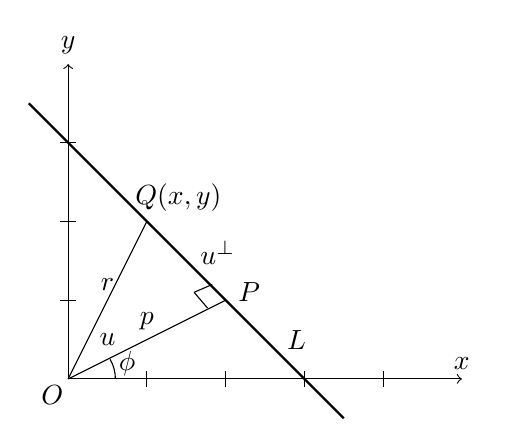
\begin{tikzpicture}
    \draw [->] (0, 0) -- (5, 0) node [above, pos=1] {$x$};
    \draw [->] (0, 0) -- (0, 4) node [above, pos=1] {$y$};

    \foreach \x in {1,2,3,4}
        \draw (\x, 0.1) -- (\x, -0.1);
    
    \foreach \y in {1,2,3}
    \draw (-0.1, \y) -- (0.1, \y);

    \draw [thick] (-0.5, 3.5) -- (3.5, -0.5);
    \node at (-0.2, -0.2) {$O$};

    \draw (0, 0) -- (2, 1) node [midway, above] {$p$};
    \draw (1.6, 1.1) -- (1.83, 1.2);
    \draw (1.6, 1.1) -- (1.77, 0.9);
    \node at (2.3, 1.1) {$P$};
    \node at (2.9, 0.5) {$L$};
    \draw (0, 0) -- (1, 2) node [pos=0.5, above] {$r$};
    \node at (1.4, 2.3) {$Q (x, y)$};
    \node at (1.9, 1.6) {$u^{\perp}$};
    \draw (0.6, 0) arc(0:30:0.5);
    \node at (0.75, 0.2) {$\phi$};
    \node at (0.5, 0.5) {$u$};
\end{tikzpicture}
\end{document}